% !TeX encoding = UTF-8
% Use XeLaTeX to compile it
%
% Эта работа распространяется на условиях лицензии Creative Commons Attribution-Noncommercial-Share Alike 3.0 New Zealand License.
% Краткое описание лицензии есть тут: http://creativecommons.org/licenses/by-nc-sa/3.0/nz/deed.ru
% Полное — там же.
% Эту книгу можно невозбранно распространять и изменять, но только соблюдая следующие условия:
% сохраняя лицензию и не вводя дополнительных ограничений, бесплатно
% и указывая авторство как оригинальной части, так и изменённой.
% Автор оригинального английского текста — Jason R Briggs http://jasonrbriggs.com/
% Автор перевода — Егор Кочетов <Egor.Kochetoff@gmail.com>
%
% This work is licensed under the Creative Commons Attribution-Noncommercial-Share Alike 3.0 New Zealand License.
% To view a copy of this license, visit http://creativecommons.org/licenses/by-nc-sa/3.0/nz
% or send a letter to Creative Commons, 171 Second Street, Suite 300, San Francisco, California, 94105, USA.
%

%TODO перевести название
\chapter{Повторное использование…}\label{ch:sortoflikerecycling}

Представь, сколько мусора ты производишь каждый день. Всякие бутылочки от воды, обёртки от еды, пакетики от овощей, пластиковые коробочки, в которых продают мясо; а ещё, возможно, журналы, газеты или другая бумага. Ну и теперь представь, что получится, если этот весь мусор сложить в одну большую кучу.

%TODO уточнить перевод
%Think about how much rubbish you create each day. Bottled water or bottles of soft drink, packets of crisps, plastic sandwich wrappers, bags of vegetables, meat on plastic trays, plastic shopping bags, newspapers, magazines, and so on and so on and so on$\ldots$
%\par
%Now just think about what would happen if all of that trash just got dumped in a pile at the end of your driveway.

\begin{center}
\includegraphics*[width=100mm]{../en/trash.eps}
\end{center}

Весь мусор, который ты выкидываешь, должен перерабатываться для повторного использования. И если повезёт, то таки перерабатывается\footnote{Если не повезёт — то просто сжигается на мусоросжигательных заводах. Это вредно и не приносит пользы, но хотя бы очищает место от мусора.}, чтобы по пути в школу не приходилось перелазить через мусорные горы. Стеклянные бутылки переплавляются в новые стеклянные ёмкости, бумагу переваривают в упаковочный картон, пластик переплавляют в более плотные пластиковые упаковки и вещи — чтобы в твоём дворе не вырастали горы ненужного мусора. Вообще, переработка мусора — весьма полезная идея, чтоб не добывать одно и то же из земли, выгрызая там дырку, а вместо этого много раз использовать уже добытое.

Нет, я не сошла с ума и я всё ещё книжка про Питон. Просто в программировании такого сорта повторное использование тоже необходимо. Не стоит набирать один и тот же код много раз: нужно использовать повторно уже написанный раньше. Это сэкономит время, а также позволит найти и убрать все ошибки только из одного кусочка кода, а не из одинаковых кусочков по всей программе (и в каком-то точно ошибка забудется когда-нибудь). Кроме того, это упрощает понимание программы при её чтении: не нужно вчитываться в один и тот же код много раз.

В Питоне (да и во многих других языках программирования) есть несколько способов повторно использовать код. Один из них мы уже встречали — в главе 3, например: там была \emph{функция} \code{range}. Функции\index{функции} пишутся один раз, а потом сколько угодно вызываются отовсюду.

Давай начнём знакомство с функциями с маленького примера:

\begin{listing}
\begin{verbatim}
>>> def myfunction(myname):
...     print('Здравствуй, %s' % myname)
...
\end{verbatim}
\end{listing}

Этот код \emph{описывает функцию} с именем \code{myfunction} и с параметром \code{myname}. \emph{Параметр}, или \emph{аргумент функции} — это обычная переменная, которой можно пользоваться внутри функции (в \emph{теле функции}), то есть внутри блока кода, который стоит после строчки, начинающейся с \code{def} (сокращения от английского \code{define}, «описывать»). Значение параметру задаётся снаружи, при вызове функции. Теперь нашу функцию можно вызвать так:

\begin{listing}
\begin{verbatim}
>>> myfunction('а где я?')
Здравствуй, а где я?
\end{verbatim}
\end{listing}

И переменная \code{myname} в функции приняла то начальное значение, которое мы написали в скобках, вызывая функцию.

Можно изменить эту функцию так, чтобы она принимала два параметра:

\begin{listing}
\begin{verbatim}
>>> def myfunction(firstname, lastname):
...     print('Привет, %s %s' % (firstname, lastname))
...
\end{verbatim}
\end{listing}

И тогда вызывать её вот так:

\begin{listing}
\begin{verbatim}
>>> myfunction('Гвидо', 'ван Россум')
Привет, Гвидо ван Россум
\end{verbatim}
\end{listing}

А можно создать переменные и передавать их в качестве значений аргументов:

\begin{listing}
\begin{verbatim}
>>> fn = 'Исаак'
>>> ln = 'Ньютон'
>>> myfunction(fn, ln)
Привет, Исаак Ньютон
\end{verbatim}
\end{listing}

Ещё функция может \emph{возвращать значение}, для этого есть слово \code{return}. Вот так это всё используется:

\begin{listing}
\begin{verbatim}
>>> def savings(chores, paper, spending):
...     return chores + paper - spending
...
>>> print(savings(10, 10, 5))
15
\end{verbatim}
\end{listing}

Функция принимает три параметра, складывает значения первых двух и вычитает значение третьего из этой суммы. Полученный результат возвращается функцией — его можно, как в примере выше, напечатать или присвоить переменной (или передать в качестве параметра другой функции):

\begin{listing}
\begin{verbatim}
>>> my_savings = savings(20, 10, 5)
>>> print(my_savings)
25
\end{verbatim}
\end{listing}

Снаружи от функции любые переменные, которые мы создаём или изменяем внутри, недоступны (хотя и есть средство, чтобы они были доступны, его использование редко оправданно):

\begin{listing}
\begin{verbatim}
>>> def variable_test():
...     a = 10
...     b = 20
...     return a * b
...
>>> print(variable_test())
200
>>> print(a)
Traceback (most recent call last):
  File "<stdin>", line 1, in <module>
NameError: name 'a' is not defined
\end{verbatim}
\end{listing} 

В примере выше мы создаём функцию \code{variable\_test}, которая умножает две переменных, объявленных в этой же функции (\code{a} и \code{b}), а потом возвращает результат. Чтобы вызвать эту функцию, надо написать её имя и пустые скобки: пустые — потому что функция не принимает параметров; но при каждом вызове любой функции надо писать скобки, чтобы отличить её от переменной. Так вот, если вызвать эту функцию, то мы получим ответ: 200. Но если после этого мы попытаемся напечатать значение переменной \code{a} (или переменной \code{b}, всё равно), то получим только ошибку. Это потому, что \emph{область видимости}\index{область видимости} переменных, значения которым присваиваются в функции, ограничена телом этой функции.

Можно себе представить функцию как маленький остров посреди океана, куда никто не приплывёт. Но иногда мимо пролетает самолёт и сбрасывает коробочку с листами бумаги: на них записаны значения аргументов функции. Островитяне что-то делают с этими аргументами, а потом результат запечатывают в бутылку и кидают в океан в нужном месте: течение потом выносит этот результат на большую землю, где и ждут ответ. И что там происходит на острове, жители большой земли не знают — какие там переменные используются, чему они равны. А вот островитяне, наоборот, могут достать свой могучий бинокль и зорко глянуть на большую землю, чтобы подсмотреть значения переменных оттуда (но поменять их не могут). Примерно так:

\begin{listing}
\begin{verbatim}
>>> x = 100
>>> def variable_test2():
...     a = 10
...     b = 20
...     return a * b * x
... 
>>> print(variable_test2())
20000
\end{verbatim}
\end{listing}

Переменные \code{a} и \code{b} созданы островитянами внутри функции и снаружи никак не видны. Переменная \code{x}, наоборот, создана снаружи (это \emph{глобальная переменная}) и видна и с острова, она влияет на результат, но точно не меняется после вызова функции.

\begin{center}
\includegraphics*[width=100mm]{../en/islanders.eps}
\end{center}

Теперь мы можем ещё вспомнить про цикл \code{for}, который мы использовали, чтобы узнать, когда сколько денег накопится. Его тоже можно добавить в функцию:

\begin{listing}
\begin{verbatim}
>>> def yearly_savings(chores, paper, spending):
...     savings = 0
...     for week in range(1, 53):
...         savings = savings + chores + paper - spending
...         print('К концу недели № %s накопится %s руб.' % (week, savings))
...
\end{verbatim}
\end{listing}

Попробуй ввести эту функцию в консоль и вызвать её с разными аргументами:

\begin{listing}
\begin{verbatim}
>>> yearly_savings (50, 100, 40)
К концу недели № 1 накопится 110 руб.
К концу недели № 2 накопится 220 руб.
К концу недели № 3 накопится 330 руб.
К концу недели № 4 накопится 440 руб.
К концу недели № 5 накопится 550 руб.
К концу недели № 6 накопится 660 руб.
К концу недели № 7 накопится 770 руб.
К концу недели № 8 накопится 880 руб.
К концу недели № 9 накопится 990 руб.
(... и так далее ...)
>>> yearly_savings (40, 120, 30)
К концу недели № 1 накопится 130 руб.
К концу недели № 2 накопится 260 руб.
К концу недели № 3 накопится 390 руб.
К концу недели № 4 накопится 520 руб.
К концу недели № 5 накопится 650 руб.
К концу недели № 6 накопится 780 руб.
К концу недели № 7 накопится 910 руб.
К концу недели № 8 накопится 1040 руб.
К концу недели № 9 накопится 1170 руб.
(... и так далее ...)
\end{verbatim}
\end{listing}

И это несколько удобнее, чем вводить заново \code{for} каждый раз, когда хочется запустить его с новыми значениями переменных.

Функции можно группировать в \emph{модули}, и это то, что делает Питон по-настоящему очень удобным, а не просто удобным. Про модули подробнее мы поговорим чуть позже.

\section{Кусочки и части}

Когда Питон устанавливается на компьютер, вместе с ним устанавливается куча его модулей и функций. Некоторые функции можно использовать прямо сразу в консоли и программах, без каких-либо специальных предварительных инструкций. Так мы использовали функцию \code{range}. Есть ещё функция \code{open}\index{функции!open}, на которую мы сейчас взглянем подробнее.

\begin{WINDOWS}

To see how \code{file} is used, open Notepad and type a few words, then save the file onto your C drive, by:

\begin{enumerate}
 \item clicking on the File menu, then Save,
 \item double-click on `My Computer' in the file dialog,
 \item double-click on `Local Drive (C:)',
 \item in the File name box (at the bottom) where it says `*.txt', type `test.txt' 
\end{enumerate}

\begin{figure}
\begin{center}
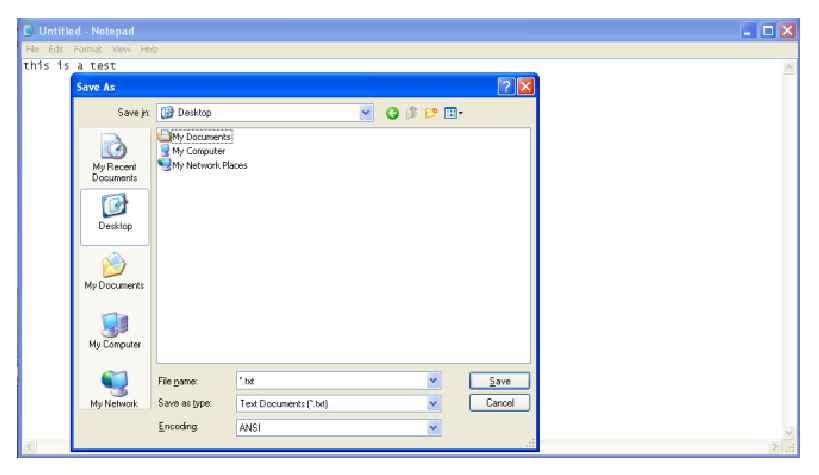
\includegraphics[width=65mm]{../en/figure17.eps}
\end{center}
\caption{The save dialog from Windows Notepad.}\label{fig17}
\end{figure}

Open the Python console again, and try the following:

\begin{listing}
\begin{verbatim}
>>> f = open('c:\\test.txt')
>>> print(f.read())
\end{verbatim}
\end{listing}

The contents of the file you just created should be printed to the console. You can now jump ahead to the bit that says: ``Continuing from here$\ldots$''.
\end{WINDOWS}

\begin{MAC}
To see how \code{file} is used, open up the Text Editor, by clicking on the editor icon (\includegraphics*[width=12mm]{../en/textedit-icon.eps}).  Type a few words then save the file to the Desktop by clicking File, then Save, and entering the name `text.txt' in the entry box next to `Save As'.

\begin{figure}
\begin{center}
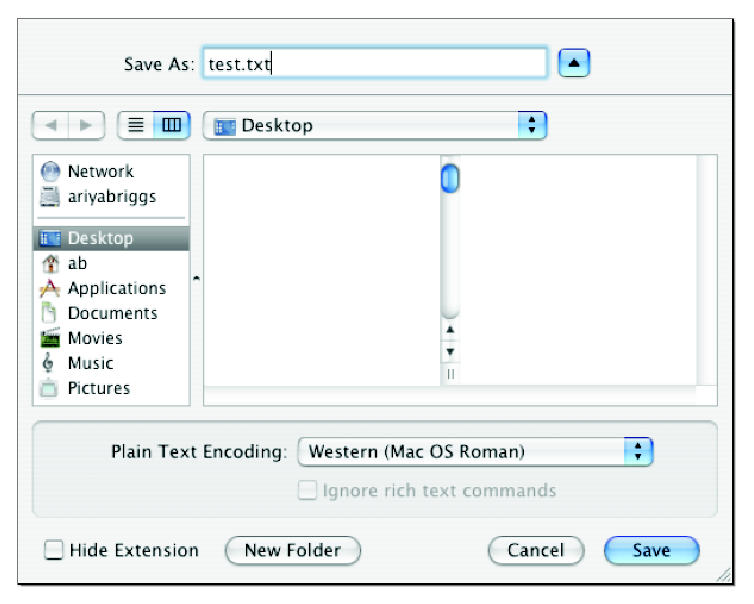
\includegraphics[width=65mm]{../en/figure18.eps}
\end{center}
\caption{The save dialog from Mac OS X Text Editor.}\label{fig18}
\end{figure}

Open the Python console again, and try the following:

\begin{listing}
\begin{verbatim}
>>> f = open('Desktop/test.txt')
>>> print(f.read())
\end{verbatim}
\end{listing}

The contents of the file you just created should be printed to the console.  You can now jump ahead to the bit that says: ``Continuing from here$\ldots$''.
\end{MAC}

\begin{LINUX}
Для этого давай откроем текстовый редактор. Напечатай туда несколько слов и сохрани этот новый файл в свою домашнюю папку, нажав, например, кнопку «сохранить» где-то слева в верху экрана (твои родители должны были показать тебе, как сохранять, где-то в первой главе) и выбрав в качестве места для cохранения домашнюю папку. Назови файл «test.txt» (должно получиться, например, как на рисунке~\ref{fig19})
	
\begin{figure}
\begin{center}
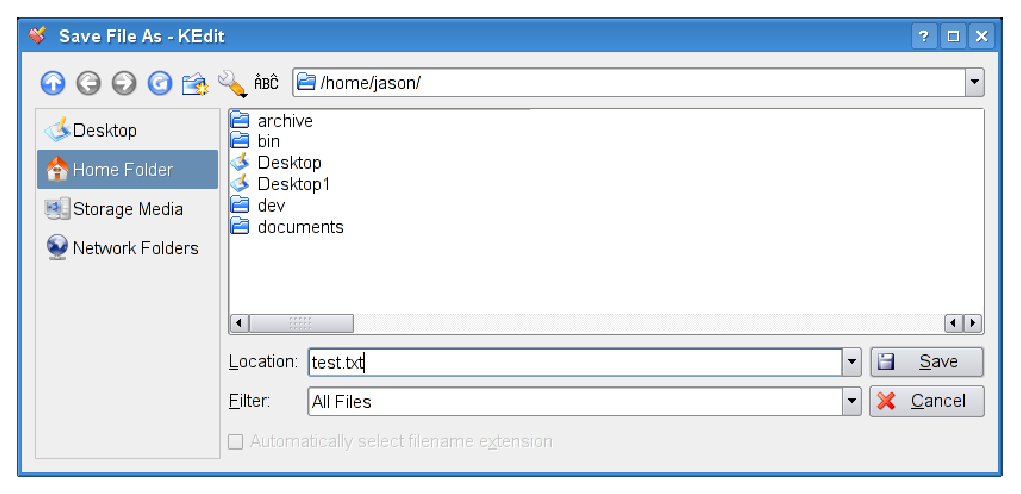
\includegraphics[width=65mm]{../en/figure19.eps}
\end{center}
\caption{Диалог сохранения может выглядеть, например, так}\label{fig19}
\end{figure}

Теперь снова открой питонью консоль и напечатай туда такие команды:

\begin{listing}
\begin{verbatim}
>>> f = open('test.txt')
>>> print(f.read())
\end{verbatim}
\end{listing}

\end{LINUX}

Давай разберёмся, что этот кусочек кода делает. Первая строка вызывает функцию \code{open}, передавая ей имя файла в качестве параметра. Эта функция открывает файл, чтобы его потом использовать. Она возвращает специальное значение (объект), которое описывает этот файл. Потом у этого объекта можно вызывать функции, чтобы прочитать что-то из файла или записать в файл. Этот объект сохраняется в переменную \code{f} в нашей строчке кода.

Потом вторая строка вызывает у объекта \code{f} функцию \code{read} (используя точку после имени объекта: именно так вызываются функции у объектов), которая читает весь файл и возвращает результат как строку. Эта строка тут же и передаётся как параметр функции \code{print}, так что весь файл печатается в консоль.

\vspace{6pt}
\begin{center}
\fbox{\colorbox{PaleBlue}{\parbox{.75\linewidth} {
В приложении~\ref{app:builtinfunctions} (в конце книжки) написано ещё всякое разное про встроенные в Питон функции.
}}}
\end{center}

\section{Модули}\index{модули}

Ну что ж, с парой способов повторно использовать код мы уже познакомились. Во-первых, это функции, которые можно и самим создавать и вызывать, и использовать встроенные в Питон (\code{range}, \code{open}, \code{int}, \code{str}). Во-вторых, можно вызывать функции у объектов — про то, как их описывать, мы потом поговорим.

Ещё можно создавать модули: файлы, содержащие функции и объекты, сгруппированные вместе. Например, всё для работы со временем содержится в модуле \code{time}\index{модули!time}. Вот так мы говорим Питону, что будем в программе использовать функции и переменные из этого модуля:

\begin{listing}
\begin{verbatim}
>>> import time
\end{verbatim}
\end{listing}

Теперь мы можем обращаться к функциям из этого модуля, используя точку (точно так же, как к функциям какого-нибудь объекта):

\begin{listing}
\begin{verbatim}
>>> print(time.localtime())
(2006, 11, 10, 23, 49, 1, 4, 314, 1)
\end{verbatim}
\end{listing}

\code{localtime}\index{модули!time!localtime} — функция, которая возвращает текущие время и дату, сохранённые в кортеже (про кортежи было во второй главе раздел «Кортежи и списки», на странице \pageref{tuplesandlists}): год, месяц, день, час, минуту, секунду, номер дня недели, номер дня года и переведены ли часы на летнее время (1, если да; 0 — если нет). Можно воспользоваться ещё одной функцией из модуля \code{time}, чтобы превратить этот кортеж в более понятную строку:

\begin{listing}
\begin{verbatim}
>>> t = time.localtime()
>>> print(time.asctime(t))
'Sun Aug 30 21:40:59 2015'
\end{verbatim}
\end{listing}

Можно это сделать в одну строку:

\begin{listing}
\begin{verbatim}
>>> print(time.asctime(time.localtime()))
'Sun Aug 30 21:41:16 2015'
\end{verbatim}
\end{listing}

А можно и ещё чуть сократить:

\begin{listing}
\begin{verbatim}
>>> time.asctime()
'Sun Aug 30 21:41:44 2015'
\end{verbatim}
\end{listing}

Потому что функция \code{asctime} как раз печатает текущее время, если никаких параметров ей не передавать.

Может случиться так, что тебе нужно будет попросить того, кто пользуется твоей программой, ввести значение. Для этого можно напечатать эту просьбу на экране и потом считать то, что твоей программе в ответ напечатают. Функция, чтобы читать то, что вводят с клавиатуры, содержится в модуле \code{sys}:

\begin{listing}
\begin{verbatim}
import sys
\end{verbatim}
\end{listing}

В этом модуле есть объект \code{stdin}\index{модули!sys!stdin} (сокращение от английского «standard input», то есть «стандартный ввод»). А у этого объекта есть функция \code{readline} — считать строку текста, то есть всё, что напечатано до нажатия клавиши Enter. Клавиша Enter заканчивает строку (точно так же, как в любом текстовом редакторе). Можешь проверить, как эта функция работает, введя вот это в консоль:

\begin{listing}
\begin{verbatim}
>>> print(sys.stdin.readline())
\end{verbatim}
\end{listing}

Напечатай что-нибудь и нажми Enter. Питон ровно эту строку и напечатает.

Теперь можем вернуться к условному оператору \code{if} из четвёртой главы. Там был такой код:

\begin{listing}
\begin{verbatim}
>>> if age >= 10 and age <= 13:
...     print('Я знаю, тебе %s лет' % age)
... else:
...     print('Столько люди не живут.')
\end{verbatim}
\end{listing}

Вместо того чтобы заранее создавать и задавать значение переменной \code{age}, можно попросить кого-то ввести возраст с клавиатуры. Но сперва давай выделим этот код в функцию:

\begin{listing}
\begin{verbatim}
>>> def your_age(age):
...     if age >= 10 and age <= 13:
...         print('Я знаю, тебе %s лет' % age)
...     else:
...         print('Столько люди не живут.')
... 
\end{verbatim}
\end{listing}

Эту функцию можно вызвать, передав ей возраст как параметр. Прежде всего, давай убедимся, что функция работает как надо:

\begin{listing}
\begin{verbatim}
>>> your_age(20)
Столько люди не живут.
>>> your_age(10)
Я знаю, тебе 10 лет
\end{verbatim}
\end{listing}

Итак, мы теперь знаем, что проблем с функцией нет — давай сделаем так, чтобы она считывала с клавиатуры, сколько человеку лет:

\begin{listing}
\begin{verbatim}
>>> def your_age():
...     print('Сколько тебе лет? Введи число и нажми Enter: ')
...     age = int(sys.stdin.readline())
...     if age >= 10 and age <= 13:
...         print('Я знаю, тебе %s лет' % age)
...     else:
...         print('Столько люди не живут.')
... 
\end{verbatim}
\end{listing}

Тут в коде вызывается функция \code{int}. Этот потому что \code{readline} возвращает текст (строку, то есть), а нам результат надо сравнить с числами, то есть использовать как число (на странице \pageref{whatsthedifference} про это подробнее). Теперь можешь потестировать эту функцию: просто вызови её.

\begin{listing}
\begin{verbatim}
>>> your_age()
Сколько тебе лет? Введи число и нажми Enter:
10
Я знаю, тебе 10 лет
>>> your_age()
Сколько тебе лет? Введи число и нажми Enter:
15
Столько люди не живут.
\end{verbatim}
\end{listing}

\btw{Да, хотя ты печатаешь вроде как число, Питон считывает строку, состоящую из цифр, но не число. Нужно не забыть превратить эту строку в число функцией \code{int}.}

\vspace{6pt}
\fbox{\colorbox{PaleBlue}{\parbox{.75\linewidth} {
\code{sys} и \code{time} — всего лишь два из кучи модулей, которые устанавливаются вместе с Питоном. Ещё про некоторые (не про все) написано в конце книжки, в приложении \ref{app:afewpythonmodules}.
}}}

\section{Что ещё попробовать}

\btw{Итак, в этой главе мы изучили, как в Питоне повторно использовать код: для этого придумали функции и модули. Мы немного обсудили область видимости переменных: что переменные, объявленные вне функции, можно использовать изнутри неё (но изменения не будут видны снаружи), а переменные, объявленные в функции, только в ней и видны. Ещё мы научились создавать функции, используя инструкцию \code{def}}.

\subsection*{Упражнение 1}
В предыдущей главе во втором упражнении мы использовали цикл \code{for}, чтобы посчитать, сколько денег накопится на нашем банковском счёте за 10 лет, если положить туда 10 000 рублей. Было бы удобно прикинуть, сколько накопится денег при других условиях. Преврати код из того упражнения в функцию, которая принимает три параметра:

\begin{enumerate}
\item Сколько денег ты кладёшь в банк;
\item На сколько лет;
\item Сколько процентов годовых обещает банк.
\end{enumerate}

В результате эту функцию должно быть можно вызвать так, и она должна давать такие ответы:

\begin{listing}
\begin{verbatim}
>>> calculate_interest (1000, 1, 11)
1110.0
>>> calculate_interest (1200, 5, 13)
2210.922215159999
>>> calculate_interest (1500, 10, 15)
6068.33660356186
\end{verbatim}
\end{listing}

\subsection*{Упражнение 3}

Вместо того чтобы задавать значения параметров из программы, лучше сделать так, чтобы функция сама их спрашивала. Тогда тому, кто будет пользоваться этой программой, надо будет просто ввести значения с клавиатуры, а не менять программный код, передавая другие значения функции (можешь спросить, например, у мамы, что ей проще).

Используй функции \code{sys.stdin.readline} и \code{int}, чтобы считывать эти данные с клавиатуры внутри функции \code{calculate\_interest}. Функцию теперь можно вызывать вот так:

\begin{listing}
\begin{verbatim}
calculate_interest()
\end{verbatim}
\end{listing}
